\documentclass[12pt, a4paper]{article}
\usepackage{geometry}
\geometry{left=2cm}
\geometry{right=1.5cm}
\geometry{top=1cm}
\geometry{bottom=2cm}
\usepackage[T1,T2A]{fontenc}
\usepackage[utf8]{inputenc}
\usepackage[english,russian]{babel}
\usepackage{amsmath}
\usepackage{amsfonts}
\usepackage{amssymb}
\usepackage{makeidx}
\usepackage{mathtext}
\usepackage{graphicx}
\graphicspath{{pictures/}}
\DeclareGraphicsExtensions{.pdf,.png,.jpg,.gif}
\begin{document}
\textit{\textbf{Кластеризация}}  —  процедура, которая собирает данные об объектах и разделяет их на группы (кластеры) по схожим признакам. Используется во многих областях: медицина, археология, маркетинг, \textit{машинное обучение} и др.\\
Нам дано множество точек, необходимо их разбить на группы по какому-либо правилу. Неизвестно, какие использовать правила, расстояния, какое количество кластеров будет в итоге. Это должны решить мы сами и исходя из наших желаний выбрать подходящий алгоритм. Рассмотрим несколько примеров расстояний, которые можно использовать в алгоритме.\\
1) Евклидово расстояние: 
\begin{equation}\label{eq:one}
\rho (x, y) = \sqrt{\sum_{i=1}^n (x_i - y_i)^2}
\end{equation}
2) Косинусное расстояние:
\begin{equation}\label{eq:two}
\rho_{cos} (x, y) = arccos({{\langle X,Y\rangle}\over{\| X \| \| Y \|}})
\end{equation}
3) Манхеттенское расстояние:
\begin{equation}\label{eq:three}
\rho (x, y) = \sum_{i=1}^n |x_i - y_i|
\end{equation}
И др.

Все алгоритмы кластеризации делятся на две большие группы: \textit{иерархические} и \textit{плоские}.\\
\textit{Иерархические} алгоритмы разделяются на восходящие и нисходящие. В восходящих предполагается, что каждый элемент, каждая точка изначально — отдельный кластер. В соответствии с введенным расстоянием и оговоренными правилами они объединяются  между собой, образуя всё большие кластеры. В нисходящих наоборот, один большой кластер в процессе алгоритма разделяется на малые. \\
\textit{Плоские} алгоритмы строят одно разбиение объектов на кластеры.

Также кластеры могут быть \textit{пересекающимися} (когда один и более элементов одного кластера одновременно могут принадлежать другим кластерам) и \textit{непересекающимися} (каждый объект принадлежит одному кластеру).
\medskip 
 \medskip 
  \medskip 
   \medskip 
   
\textit{\textbf{Алгоритм k-средних.}}\\Для этого алгоритма необходимо задать необходимое количество кластеров до начала его исполнения. На каждой итерации вычисляется центр масс каждого кластера, полученного на предыдущем шаге. После этого происходит перераспределение объектов относительно нового положения центров масс, далее вычисляются новые положения центров масс и тд. Так происходит до момента, пока кластеры не найдут свое «устойчивое» положение, то есть, когда при каждой следующей итерации центры масс не меняют своего положения или меняют, менее чем на на $\epsilon$, который мы задали. Сложность алгоритма по времени, нужному для сходимости, равна $2^{\Omega(\sqrt{n})}.$
\begin{figure}[h!]
\center{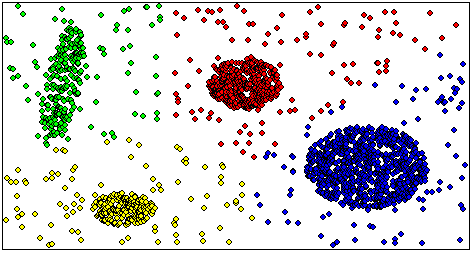
\includegraphics{k-means}}
\caption{Результат работы алгоритма k-средних.}
\label{fig:k}
\end{figure}
\medskip 
 \medskip 
  \medskip 
   \medskip 
   
\textit{\textbf{Алгоритм DBSCAN.}}\\Density-based spatial clustering of applications with noise (плотностной алгоритм пространственной кластеризации с присутствием шума). Алгоритм вычисляет расстояния между всеми точками. До начала работы алгоритма задаем максимальное расстояние, при котором считаем две точки «соседями», то есть, они расположены достаточно близко друг к другу. Также задаем минимальное количество точек в кластере заранее (возьмем это число за N). Поэтому после работы алгоритма имеем информацию, сколько «соседей» у каждой из точек. Теперь возможны три варианта:\\1) У точки N и более «соседей», которые вместе образуют кластер.\\2) У точки есть «соседи», их меньше N, но хотя бы один из «соседей» принадлежит кластеру. Такие точки считаются граничными с кластером, но ему всё равно не принадлежат.\\3) У точки нет «соседей» или их меньше, чем N, но ни один из них не принадлежит кластеру. Такая точка считается шумом, не принадлежит кластеру.\\После выполнения алгоритма имеем картину с кластерами, их граничными точками и шумом. Время работы: $\mathcal{O}(n*log(n)).$
\begin{figure}[h!]
\center{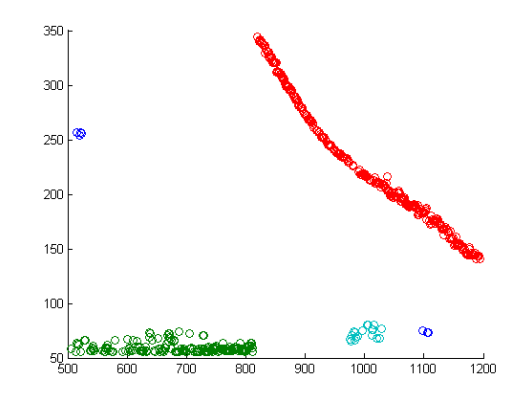
\includegraphics{dbscan}}
\caption{Результат работы алгоритма DBSCAN.}
\label{fig:dbscan}
\end{figure}
\medskip 
 \medskip 
  \medskip 
   \medskip 
   
\textit{\textbf{Иерархический алгоритм.}}

Изначально все точки считаем отдельными кластерами. До начала работы необходимо задать количество кластеров, которое хотим получить после завершения алгоритма, иначе все точки объединятся в один кластер. Далее придумываем признак, по которому будем объединять кластеры. Например, объединяем кластеры, между центрами масс которых минимальное расстояние.
 На каждой итерации происходит объединение кластеров и пересчет центра масс (если использовать предложенный признак) и завершается алгоритм по достижении нужного количества кластеров. 
 \begin{figure}[h!]
\center{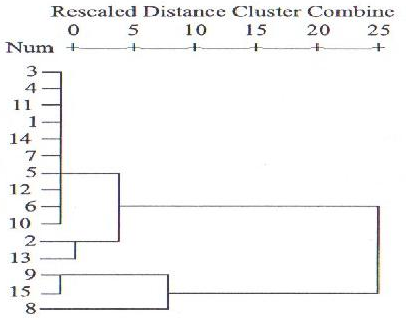
\includegraphics{dendrogr}}
\caption{Результат работы иерархического алгоритма можно представить как дендрограмму.}
\label{fig:dbscan}
\end{figure}
\end{document}